\section{Results}

\subsection{Scenario analysis}

Figure \ref{fig:scenarios_overview} shows the range of benefit, measured by utility or the proportion of patients with an outcome of mRS 0--2, across all of the scenarios to explore the effect of changing the process durations, with changes shown both separately for nLVO and LVO and for a combination assuming 70\% nLVO and 30\% LVO in the treated population.
For the combined nLVO/LVO population, compared with usual care, MSU care has a net improvement in:
the proportion of patients with an outcome of mRS 0--2 and a net improvement in utility for 92\% of all scenarios;
the proportion of patients with an outcome of mRS 0--2 of at least 0.01, 0.02, 0.03, or 0.04 in 77\%, 53\%, 29\%, and 11\% of all scenarios respectively;
and utility of at least 0.01, 0.02, 0.03, or 0.04 in 75\%, 49\%, 23\%, and 7\% of all scenarios respectively.
Across the majority of scenarios the benefit of MSU care over usual care was typically (interquartile range across scenarios) an improvement of the proportion of patients mRS 0--2 of 0.005 to 0.023 for nLVO, 0.017 to 0.055 for LVO treated with both IVT and MT, and 0.011 to 0.032 for the combined population. This translated to an improvement of 0.005 to 0.021 in utility for nLVO, 0.016 to 0.052 for LVO treated with both IVT and MT, and 0.010 to 0.029 for the combined population. 
The benefit to patients with LVO was derived mostly by increasing the benefit from MT due to faster treatment times after direct transport to a CSC.
% NOTE - haven't we just said the following? - 
% For the combined population there was typically (interquartile range across scenarios) an improvement of 0.010 to 0.029 in utility, and an improvement of 0.011 to 0.032 for the proportion of patients with an outcome of mRS 0--2.

\begin{figure}[h!]
    \centering
    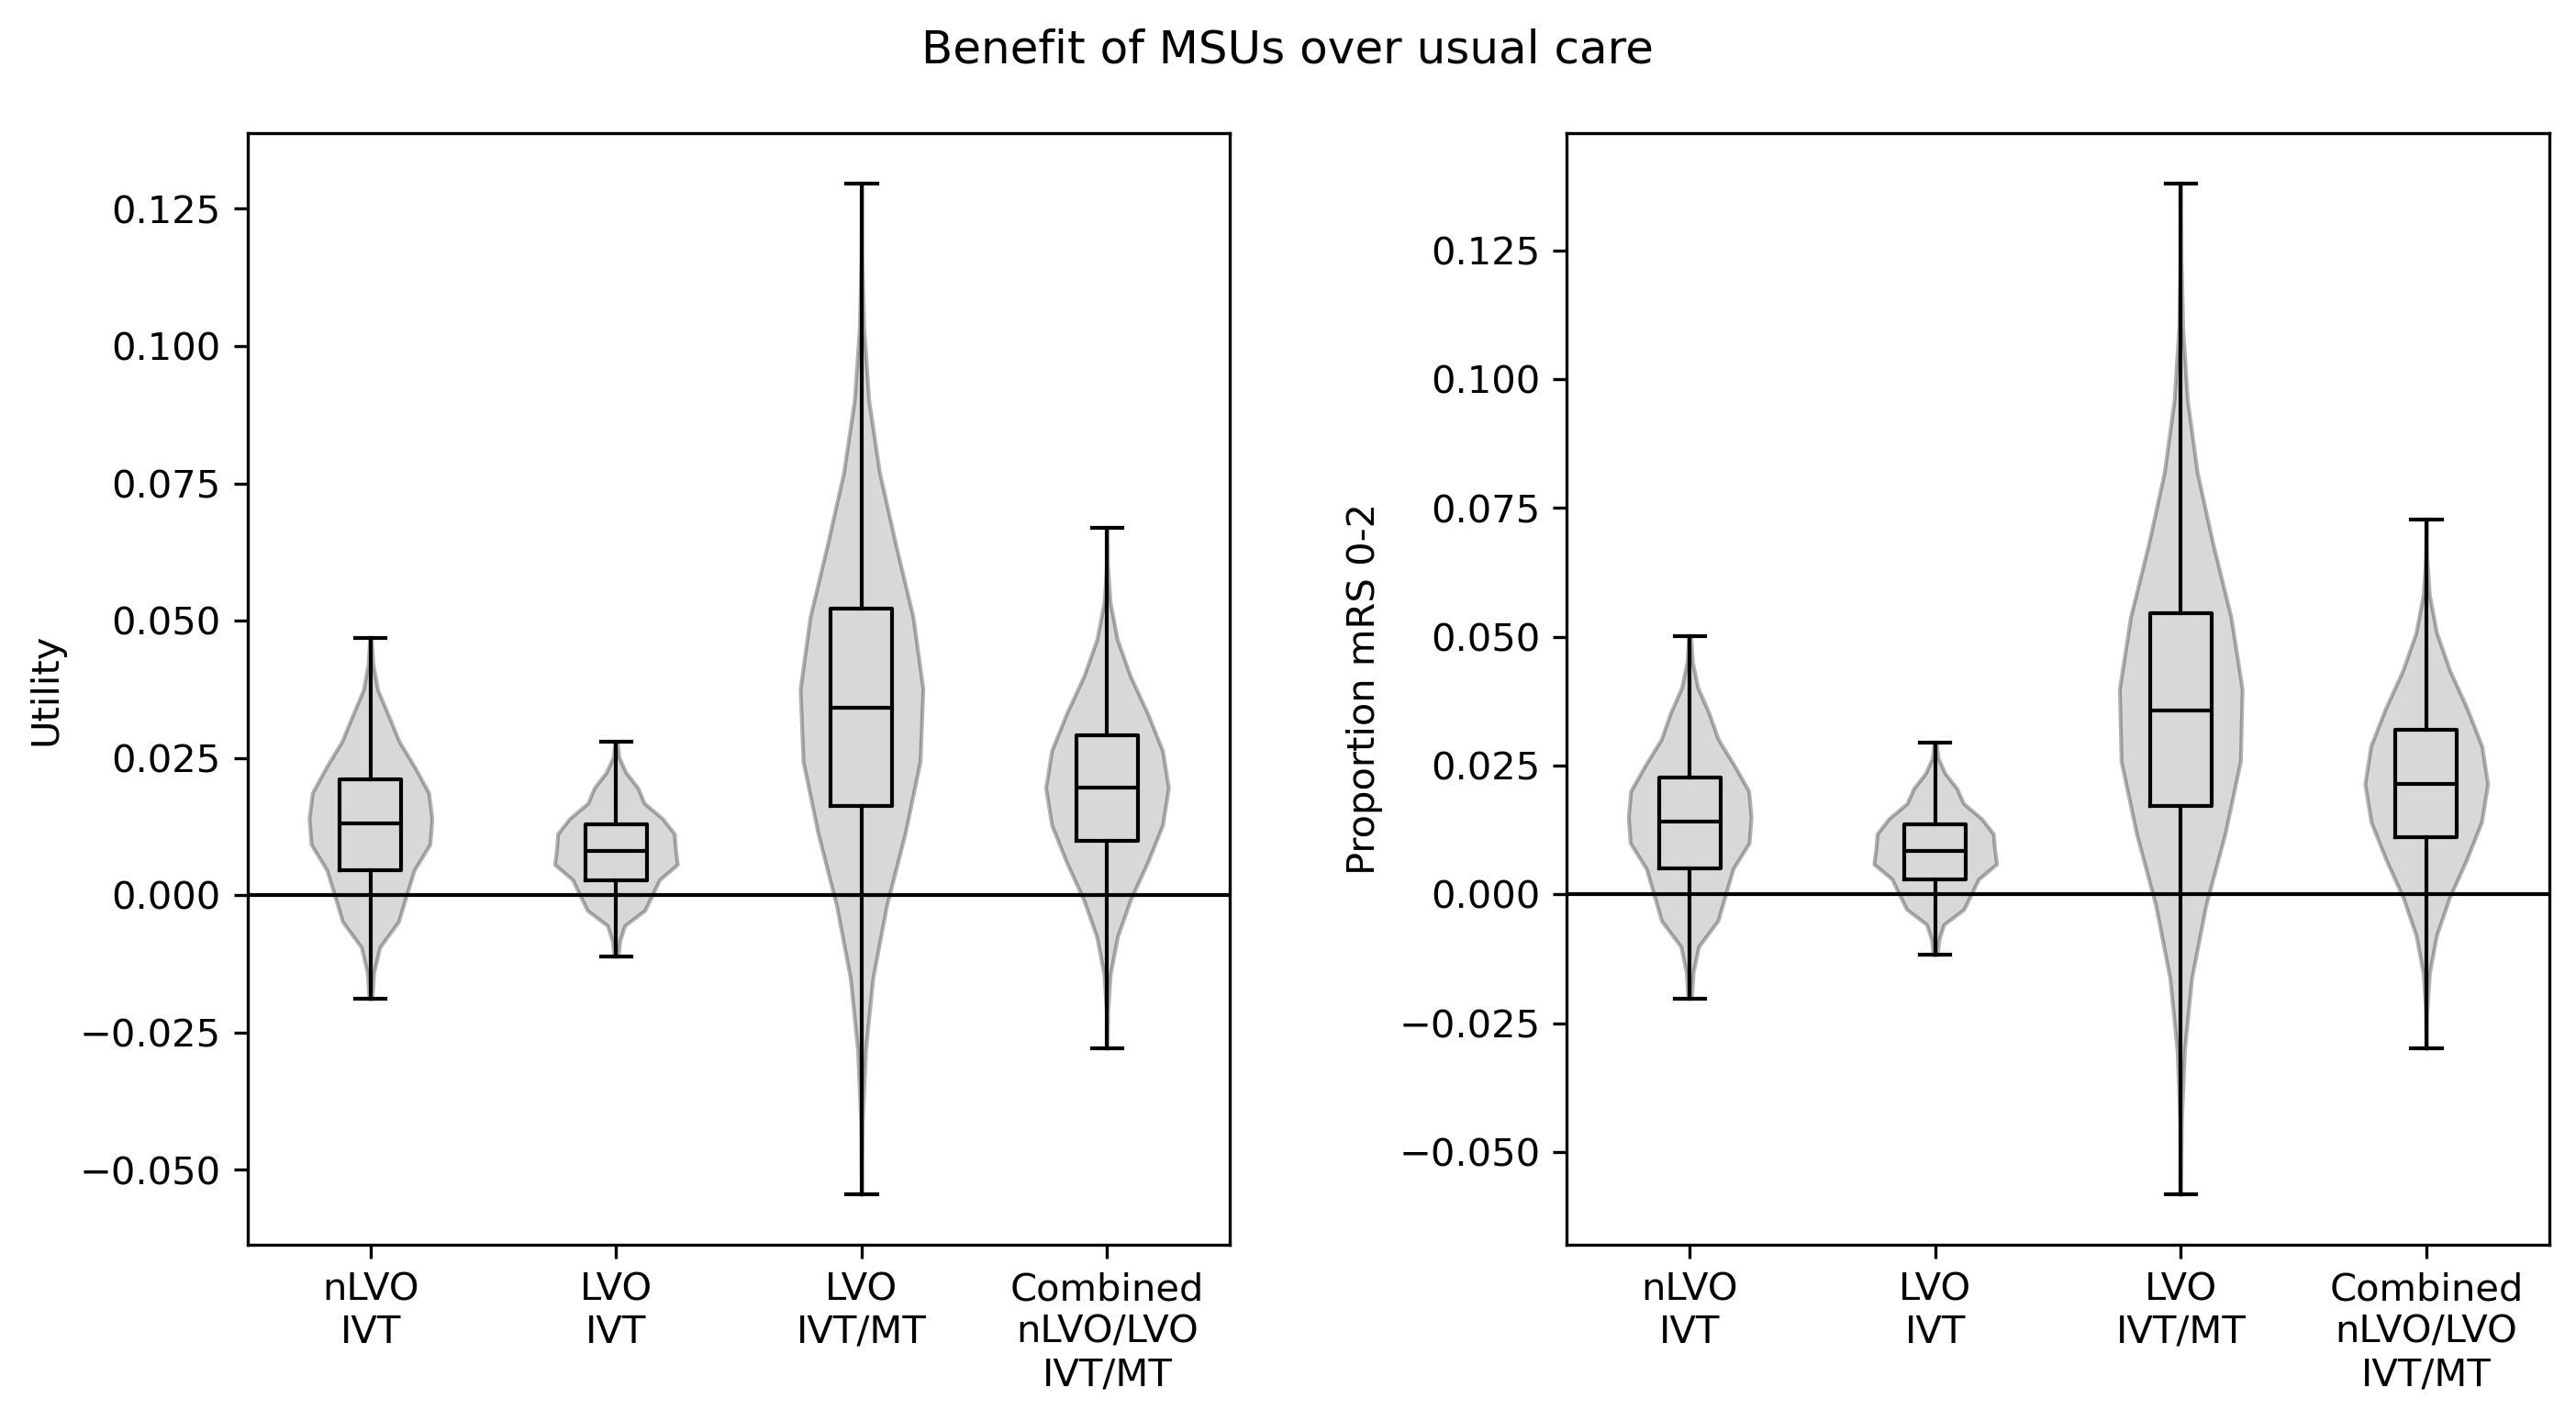
\includegraphics[width=0.75\linewidth]{images/scenario_results_summary.png}
    \caption{Benefit of MSU care over usual care across all scenarios (exploring the effect of changing process durations), in the treated population, measured by utility (left) or the proportion of patients with an outcome of mRS 0--2 (right), separating the changes for patients with nLVO and LVO. Results for LVO patients show the effect of MSU care on the benefit derived from IVT alone, or by IVT/MT in combination. Box plots show range, interquartile range, and median across all scenarios. The combined nLVO/LVO benefit assumed 70\% nLVO and 30\% LVO in the treated population, with LVOs receiving IVT/MT in combination. Overlaid on the box plots are violin plots showing the distribution of results across all scenarios. A positive value indicates MSU care provides an advantage over usual care, and a negative value indicates MSU care is disadvantageous compared with usual care. Results are the average effect across all LSOAs in England.}
    \label{fig:scenarios_overview}
\end{figure}

Figures \ref{fig:scenarios_mrs}  and \ref{fig:scenarios_utility} show how changing modelled process durations affects the predicted benefit of MSU care, expressed in proportion of patients with an outcome of mRS 0--2 or utility, respectively. Results show the combined effect on nLVO/LVO, with patients with LVO receiving IVT/MT in combination. Changing time from onset to call only had marginal effect on the benefit of MSU care over usual care. Changing parameters that worsen usual care (such as lengthening ambulance response times, or lengthening arrival to IVT), lead to increased advantages of MSU care over usual care. Likewise, changing parameters that improve MSU care (such as MSU dispatch times, or time to IVT on scene) increased the advantages of MSU care over usual care.

\begin{figure}[h!]
    \centering
    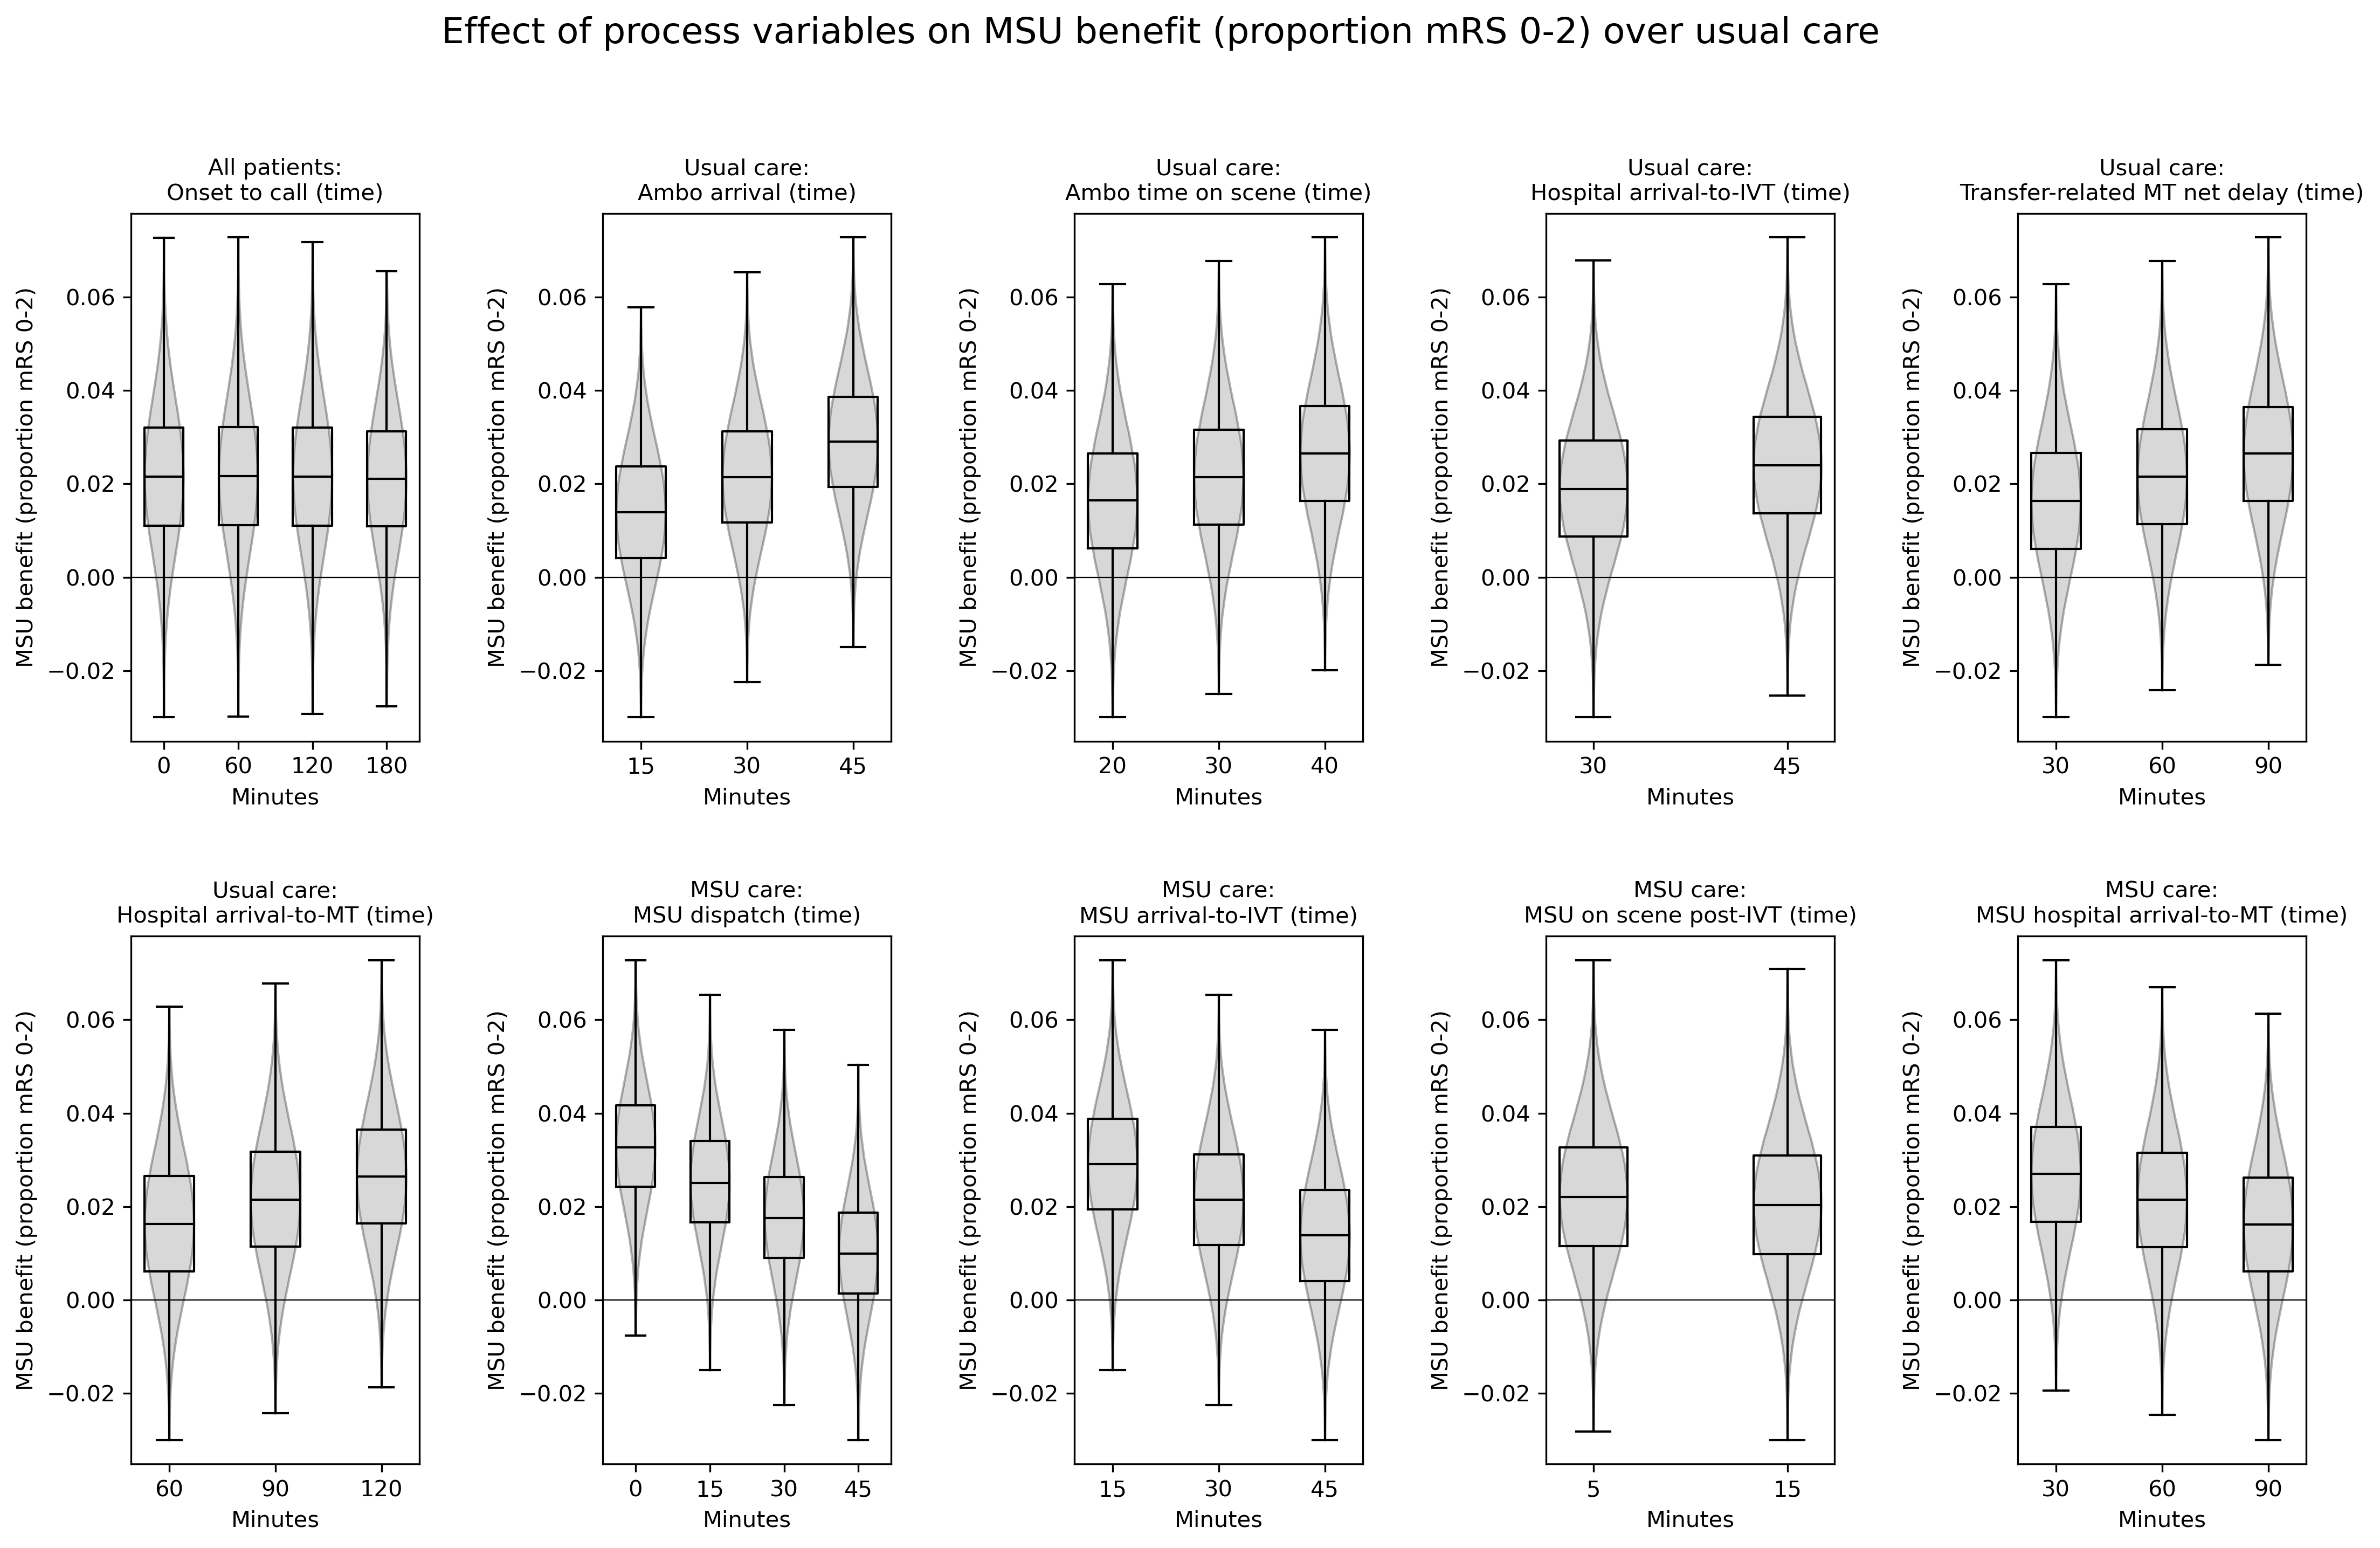
\includegraphics[width=1\linewidth]{images/msu_net_mrs_0-2_benefit.png}
    \caption{The effect of changing modelled process durations on the predicted benefit of MSU care over usual care, in the treated population (comprised of 70\% nLVO and 30\% LVO patients, where nLVO patients receive IVT and LVO patients receive IVT followed by MT), measured by proportion of patients with an outcome of mRS 0--2. For each target parameter, results are averaged across all scenarios with that given parameter value. Box plots show range, interquartile range, and median, across all scenarios. Overlaid over the box plots are violin plots showing the distribution of results across all scenarios. Results are the average effect across all LSOAs in England.}
    \label{fig:scenarios_mrs}
\end{figure}

\begin{figure}[h!]
    \centering
    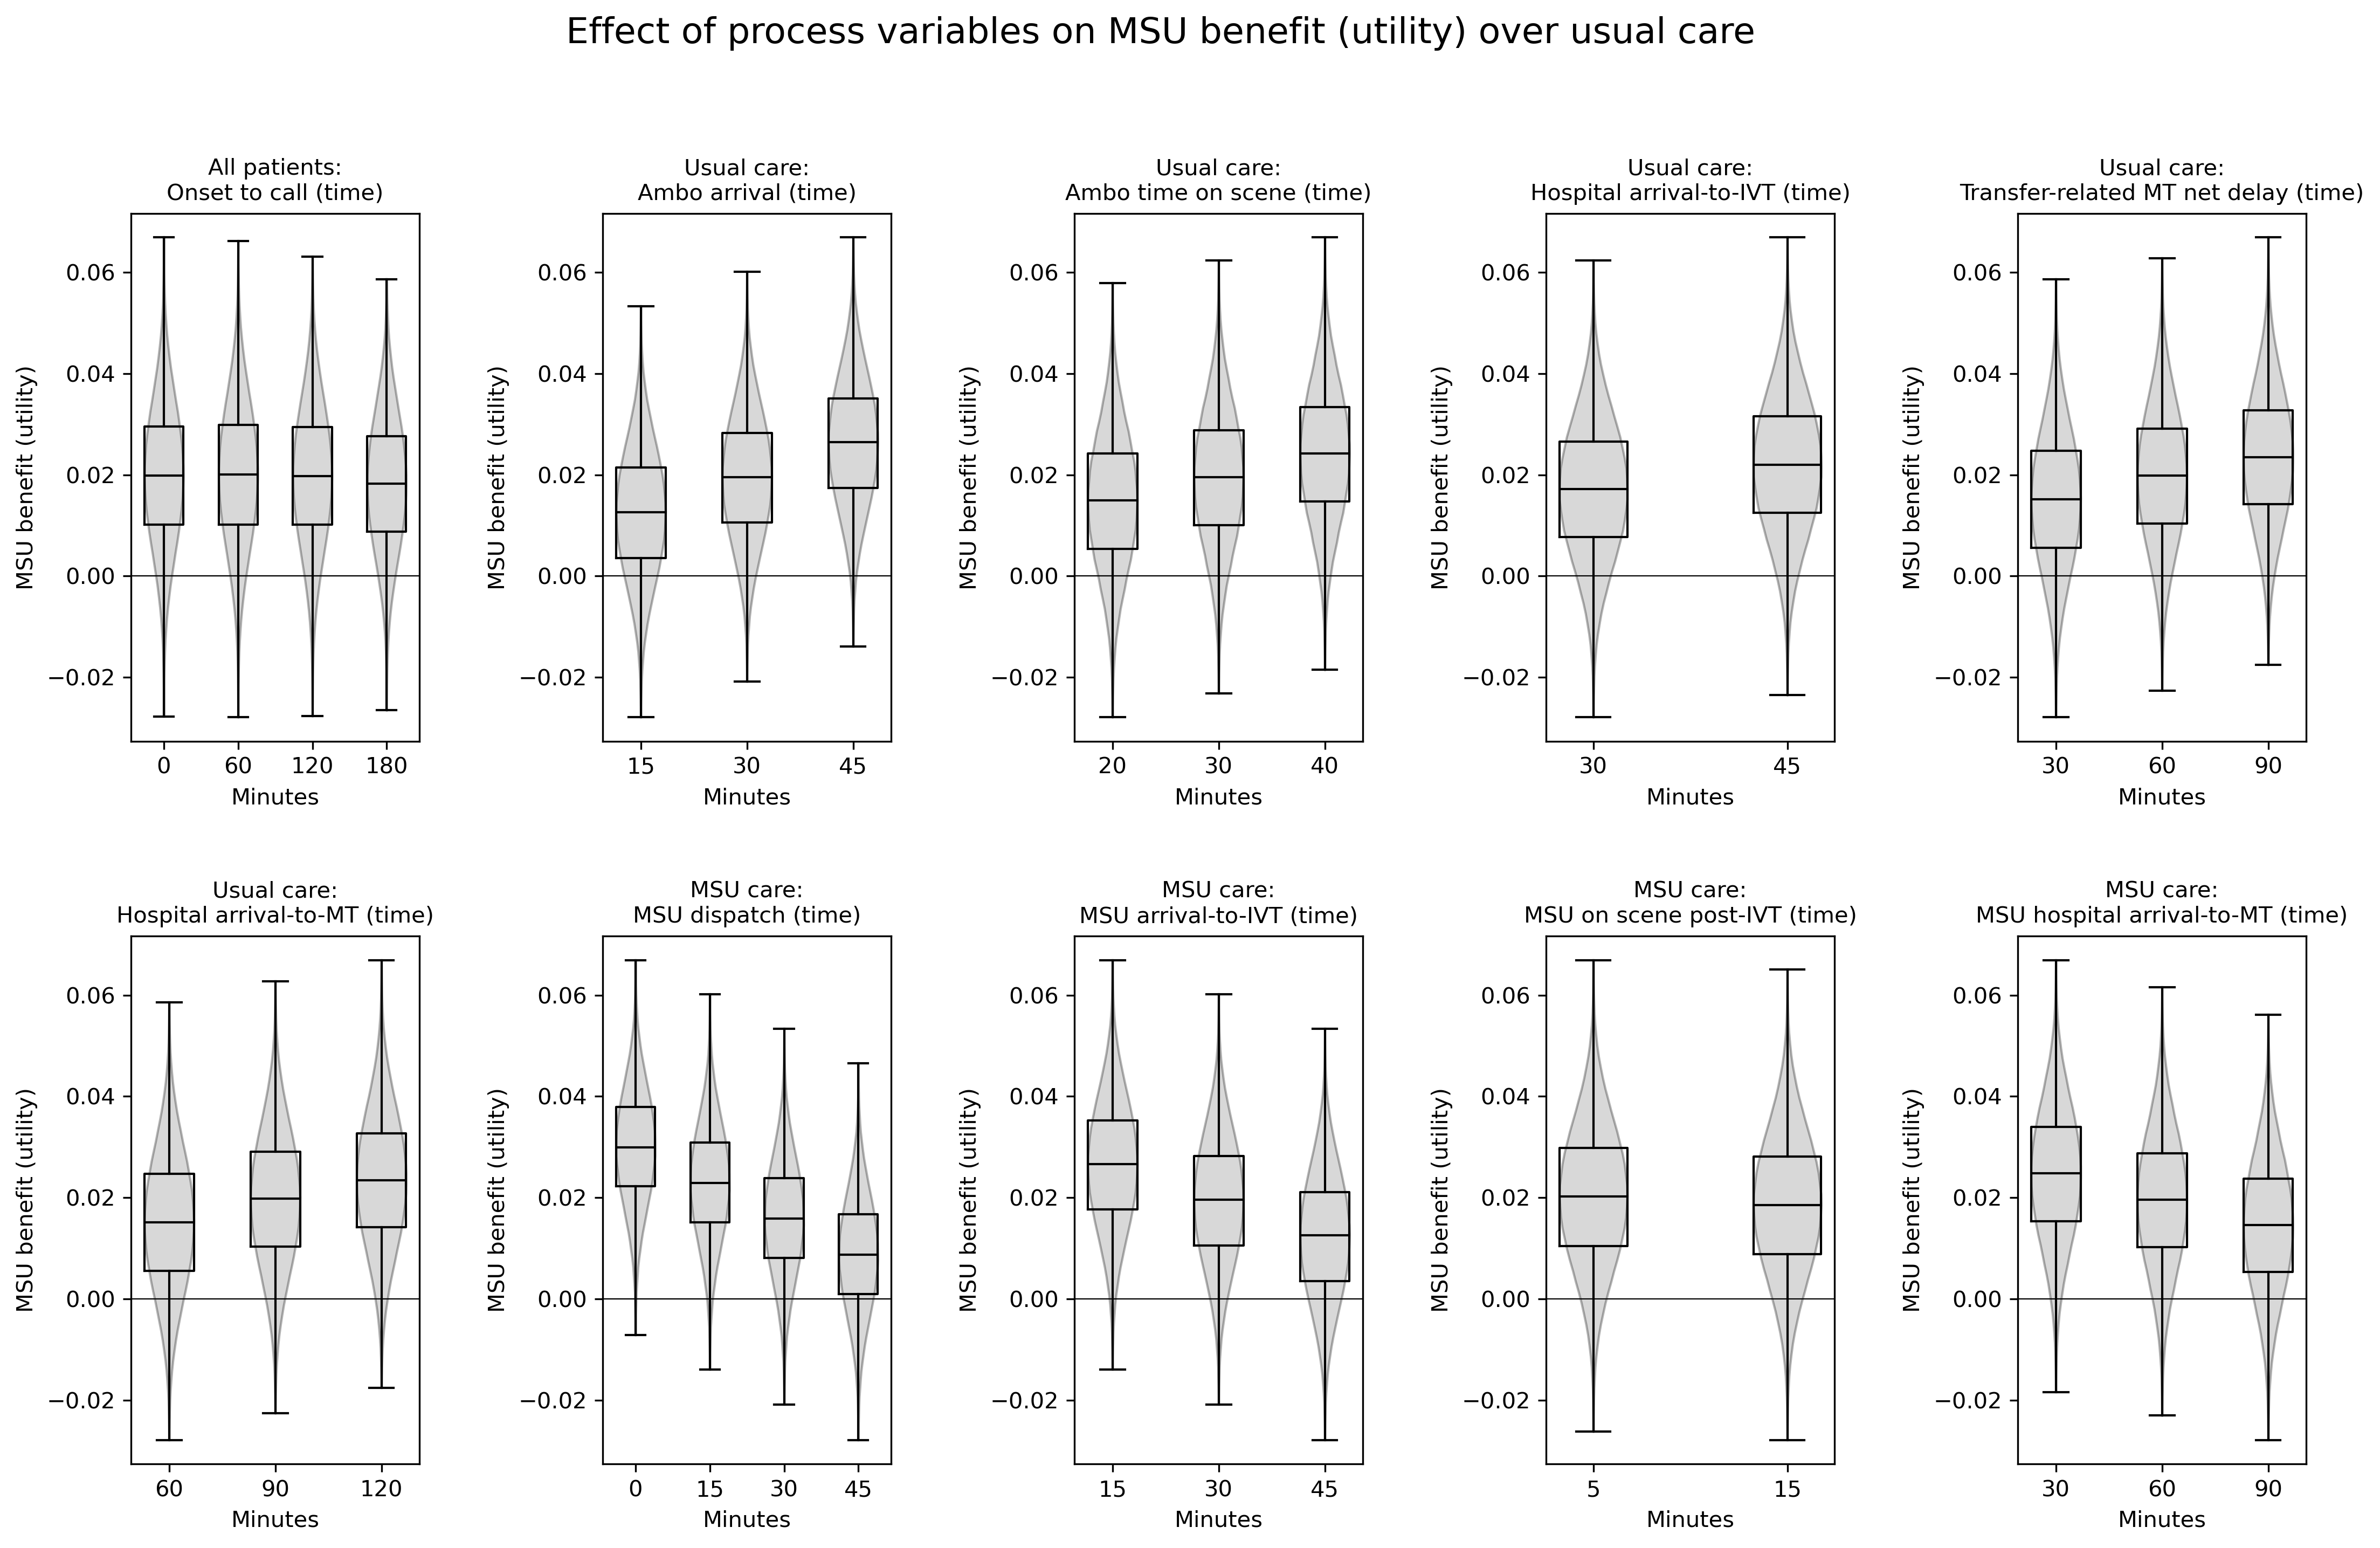
\includegraphics[width=1\linewidth]{images/msu_net_utility_benefit.png}
    \caption{The effect of changing modelled process durations on the predicted benefit of MSU care over usual care, in the treated population (comprised of 70\% nLVO and 30\% LVO patients, where nLVO patients receive IVT and LVO patients receive IVT followed by MT), measured by utility. For each target parameter, results are averaged across all scenarios with that given parameter value. Box plots show range, interquartile range, and median, across all scenarios. Overlaid over the box plots are violin plots showing the distribution of results across all scenarios. Results are the average effect across all LSOAs in England.}
    \label{fig:scenarios_utility}
\end{figure}

\subsection{Geographic variation}

For this comparison, the MSUs are based at CSCs only and we assume there is a mix of 70\% nLVO and 30\% LVO in the treated population in which nLVO patients receive IVT and LVO patients receive IVT followed by MT.

Figure \ref{fig:map_times} shows travel and transfer times for usual care and for MSU care. Under usual care, when a patient first attends a PSC (providing only IVT), the travel/transfer time to MT include the travel time to the nearest PSC, and a net additional 60 minute delay (taking into account the \textit{door-in-door-out} time at the first admitting hospital and a reduction in time to MT at the CSC for transferred patients). Under usual care, there is significant variation in travel times from patient LSOA to the first attended centre (PSC or CSC) for IVT, but there is more substantial variation in times to MT due to some patients (67\% of LSOAs and 70\% of admissions) requiring a transfer for MT. Under MSU care, as the MSUs are based at CSCs only, travel times for an MSU to deliver IVT can exceed the travel time of a normal ambulance to the closest centre providing IVT, and this extra travel time can lead to delayed time to IVT in those LSOAs furthest away from MSU base locations. However, for patients living in LSOAs that are close to a CSC, but with a PSC even closer, these patients benefit from MT sooner under MSU care than compared to usual care as they avoid the delays relating to attending the PSC first.

\begin{figure}[h!]
    \centering
    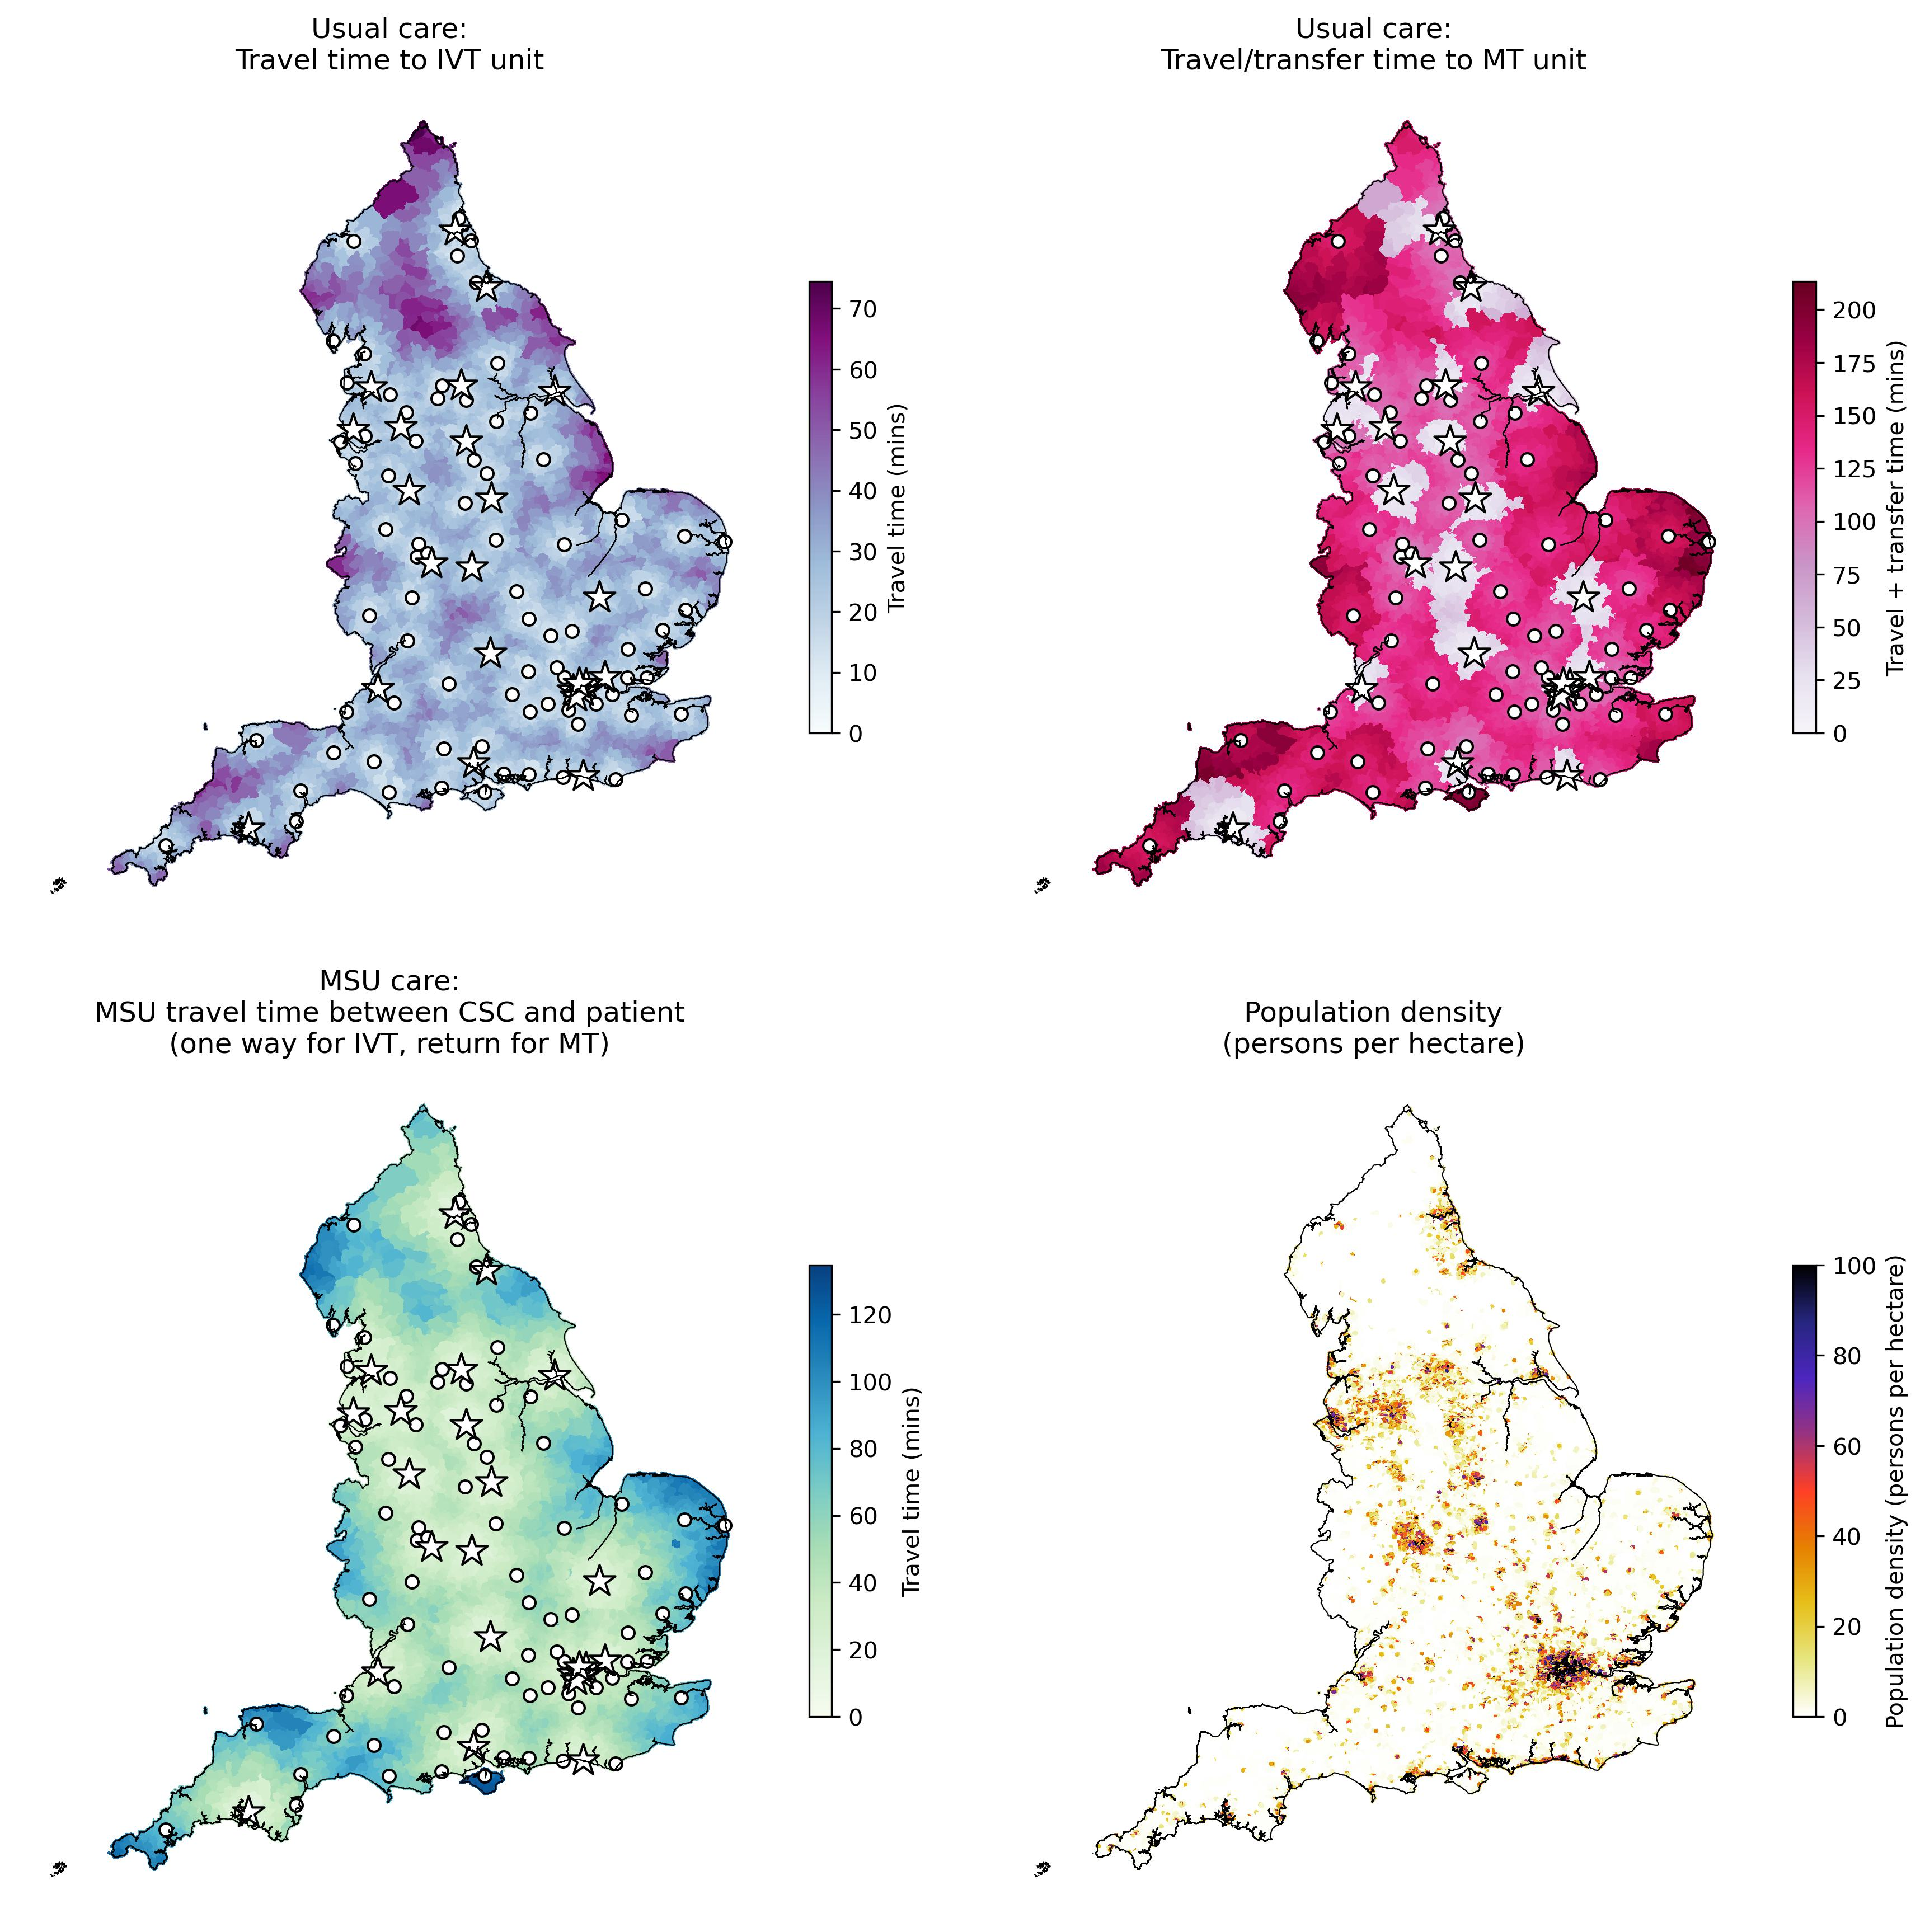
\includegraphics[width=1.0\linewidth]{images/map_times.jpg}
    \caption{Travel times to treatment under the two treatment delivery models, and population density for each LSOA. \textit{Top left}: With \emph{usual care} the travel times from the patients LSOA to their nearest PSC (providing only IVT). \textit{Top right}: With \emph{usual care} the travel and, where necessary, transfer times from the patients LSOA to a CSC (providing MT). For those patients that first attend a PSC providing only IVT, the times shown include the travel time to the PSC, a net additional delay of 60 minutes, and the inter-hospital travel time between PSC and CSC. \textit{Bottom left}: With \emph{MSU care} with the MSU base locations at the current 23 CSCs, the travel times for the MSU between the patients LSOA and their nearest CSC (one way for travel time to IVT, return journey for travel time to MT). \textit{Bottom right}: Population density (with scale capped at 100 persons per hectare). Circles show locations of PSCs (providing only IVT). Stars show locations of CSCs (providing both IVT and MT), and being the base locations of MSUs.}
    \label{fig:map_times}
\end{figure}

Figures \ref{fig:msu_map_mrs_0_2} and \ref{fig:msu_map_utility} show maps (by ischaemic stroke subtype) of geographic variation in benefit (expressed in proportion of patients with an outcome of mRS 0--2 or utility, respectively) between treatment delivery models. Overall, with no reperfusion treatment, there is an average outcome utility of 0.52 across the combined population. With usual care, there is a utility gain of 0.086 in treated patients. MSU care provided an average further utility gain in treated patients of 0.022 over usual care. There is significant variation in the benefit of reperfusion using usual care, with those living closest to CSCs receiving the greatest benefit. This is due to the larger utility gain of reperfusion treatment coming from the treatment of LVO, and with those patients benefiting most from rapid access to MT.

The benefit of MSU care over usual care follows different patterns for nLVO and LVO patients. For nLVO patients, the benefit of MSU care decreases with increased distance from the MSU base location. For LVO patients the benefit of MSU care first decreases with increased distance from the MSU base location, but then benefit increases where use of the MSU avoids inter-hospital transfer for MT, before decreasing again with greater travel times for the MSU. The catchment area of benefit for LVO under MSU care is therefore wider than the catchment area of benefit for nLVO, with the maximum benefit being in a halo a little distance from the MSU base location, where patient transfer for MT is avoided but MSU travel times are still acceptable.

\begin{figure}[h!]
    \centering
    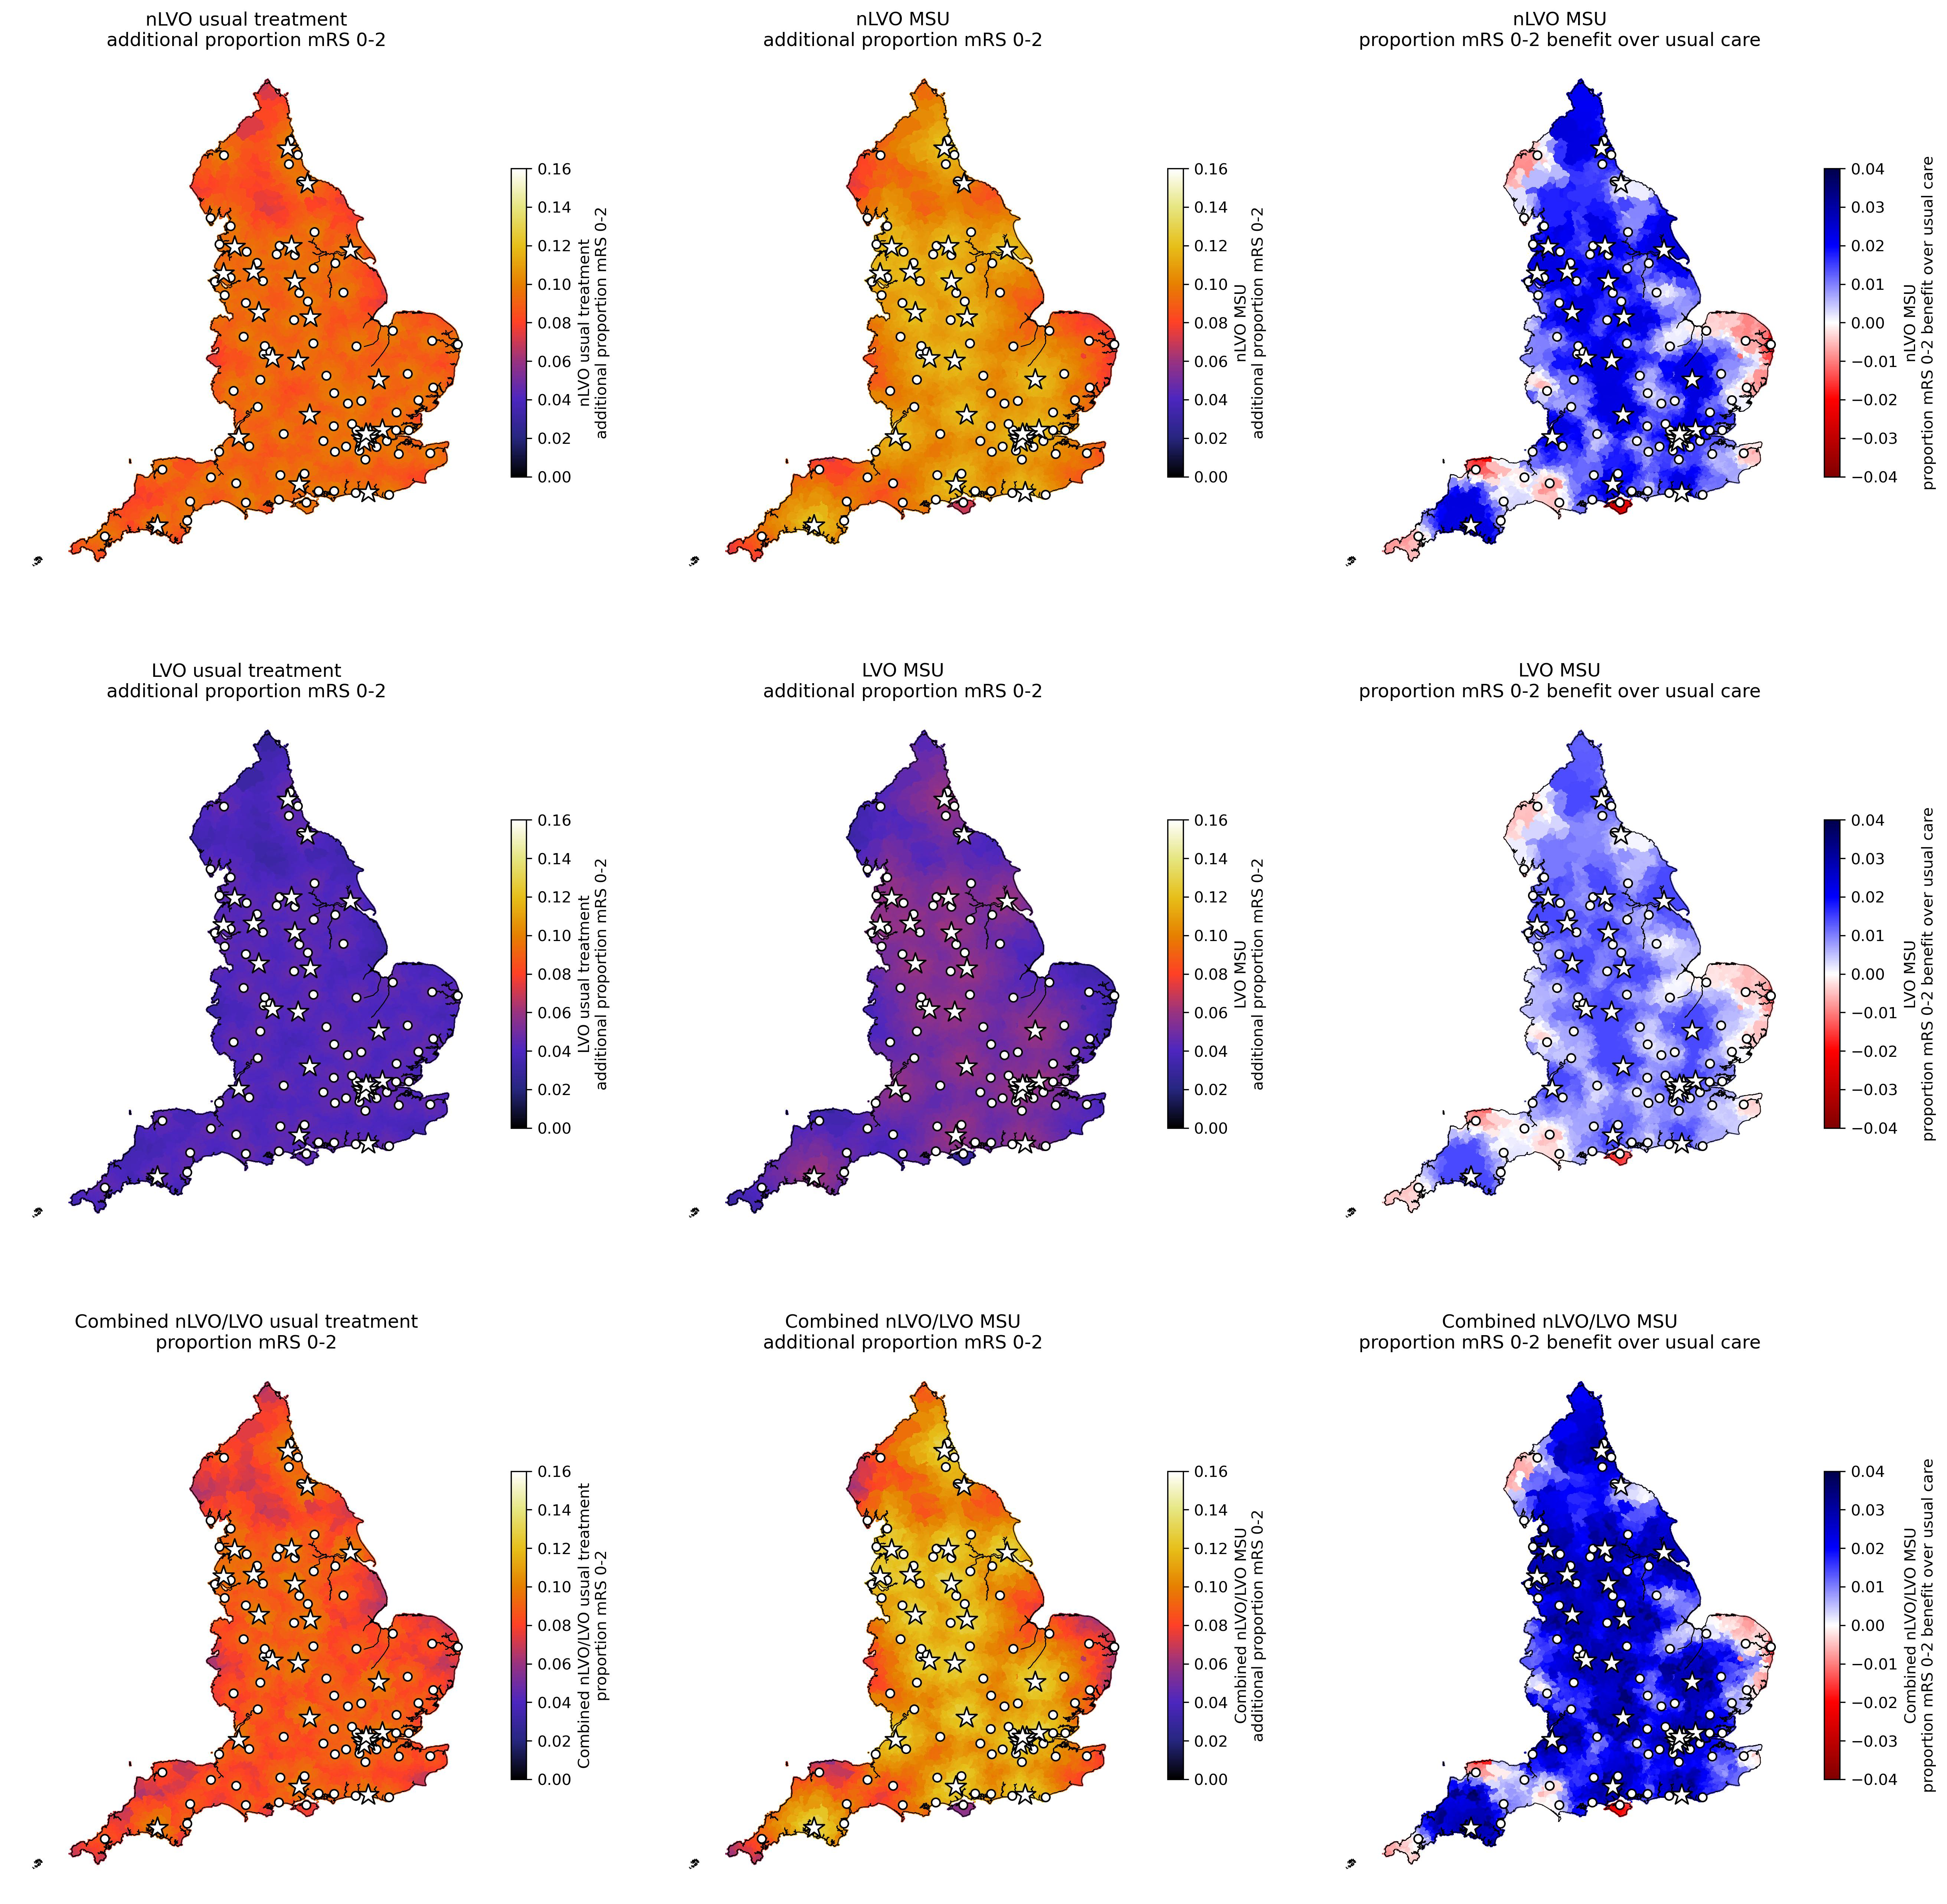
\includegraphics[width=1\linewidth]{images/map_mrs_0_2.jpg}
    \caption{Map of treatment benefits expressed as the proportion of patients with an outcome of mRS 0--2, calculated by LSOA for the treated population. \textit{Top}: Treatment of nLVO; \textit{Middle}: Treatment of LVO, \textit{Bottom}: Combination of treatment (based on 70\% nLVO and 30\% LVO in the treated population, with LVO receiving IVT/MT in combination). \textit{Left}: Benefit of usual care over no treatment; \textit{Middle}: Benefit of MSU care over no treatment; \textit{Right}: Benefit of MSU care over usual care. Circles show locations of PSCs (providing only IVT). Stars show locations of CSCs (providing both IVT and MT, and are also the base locations of MSUs).}
    \label{fig:msu_map_mrs_0_2}
\end{figure}

\begin{figure}[h!]
    \centering
    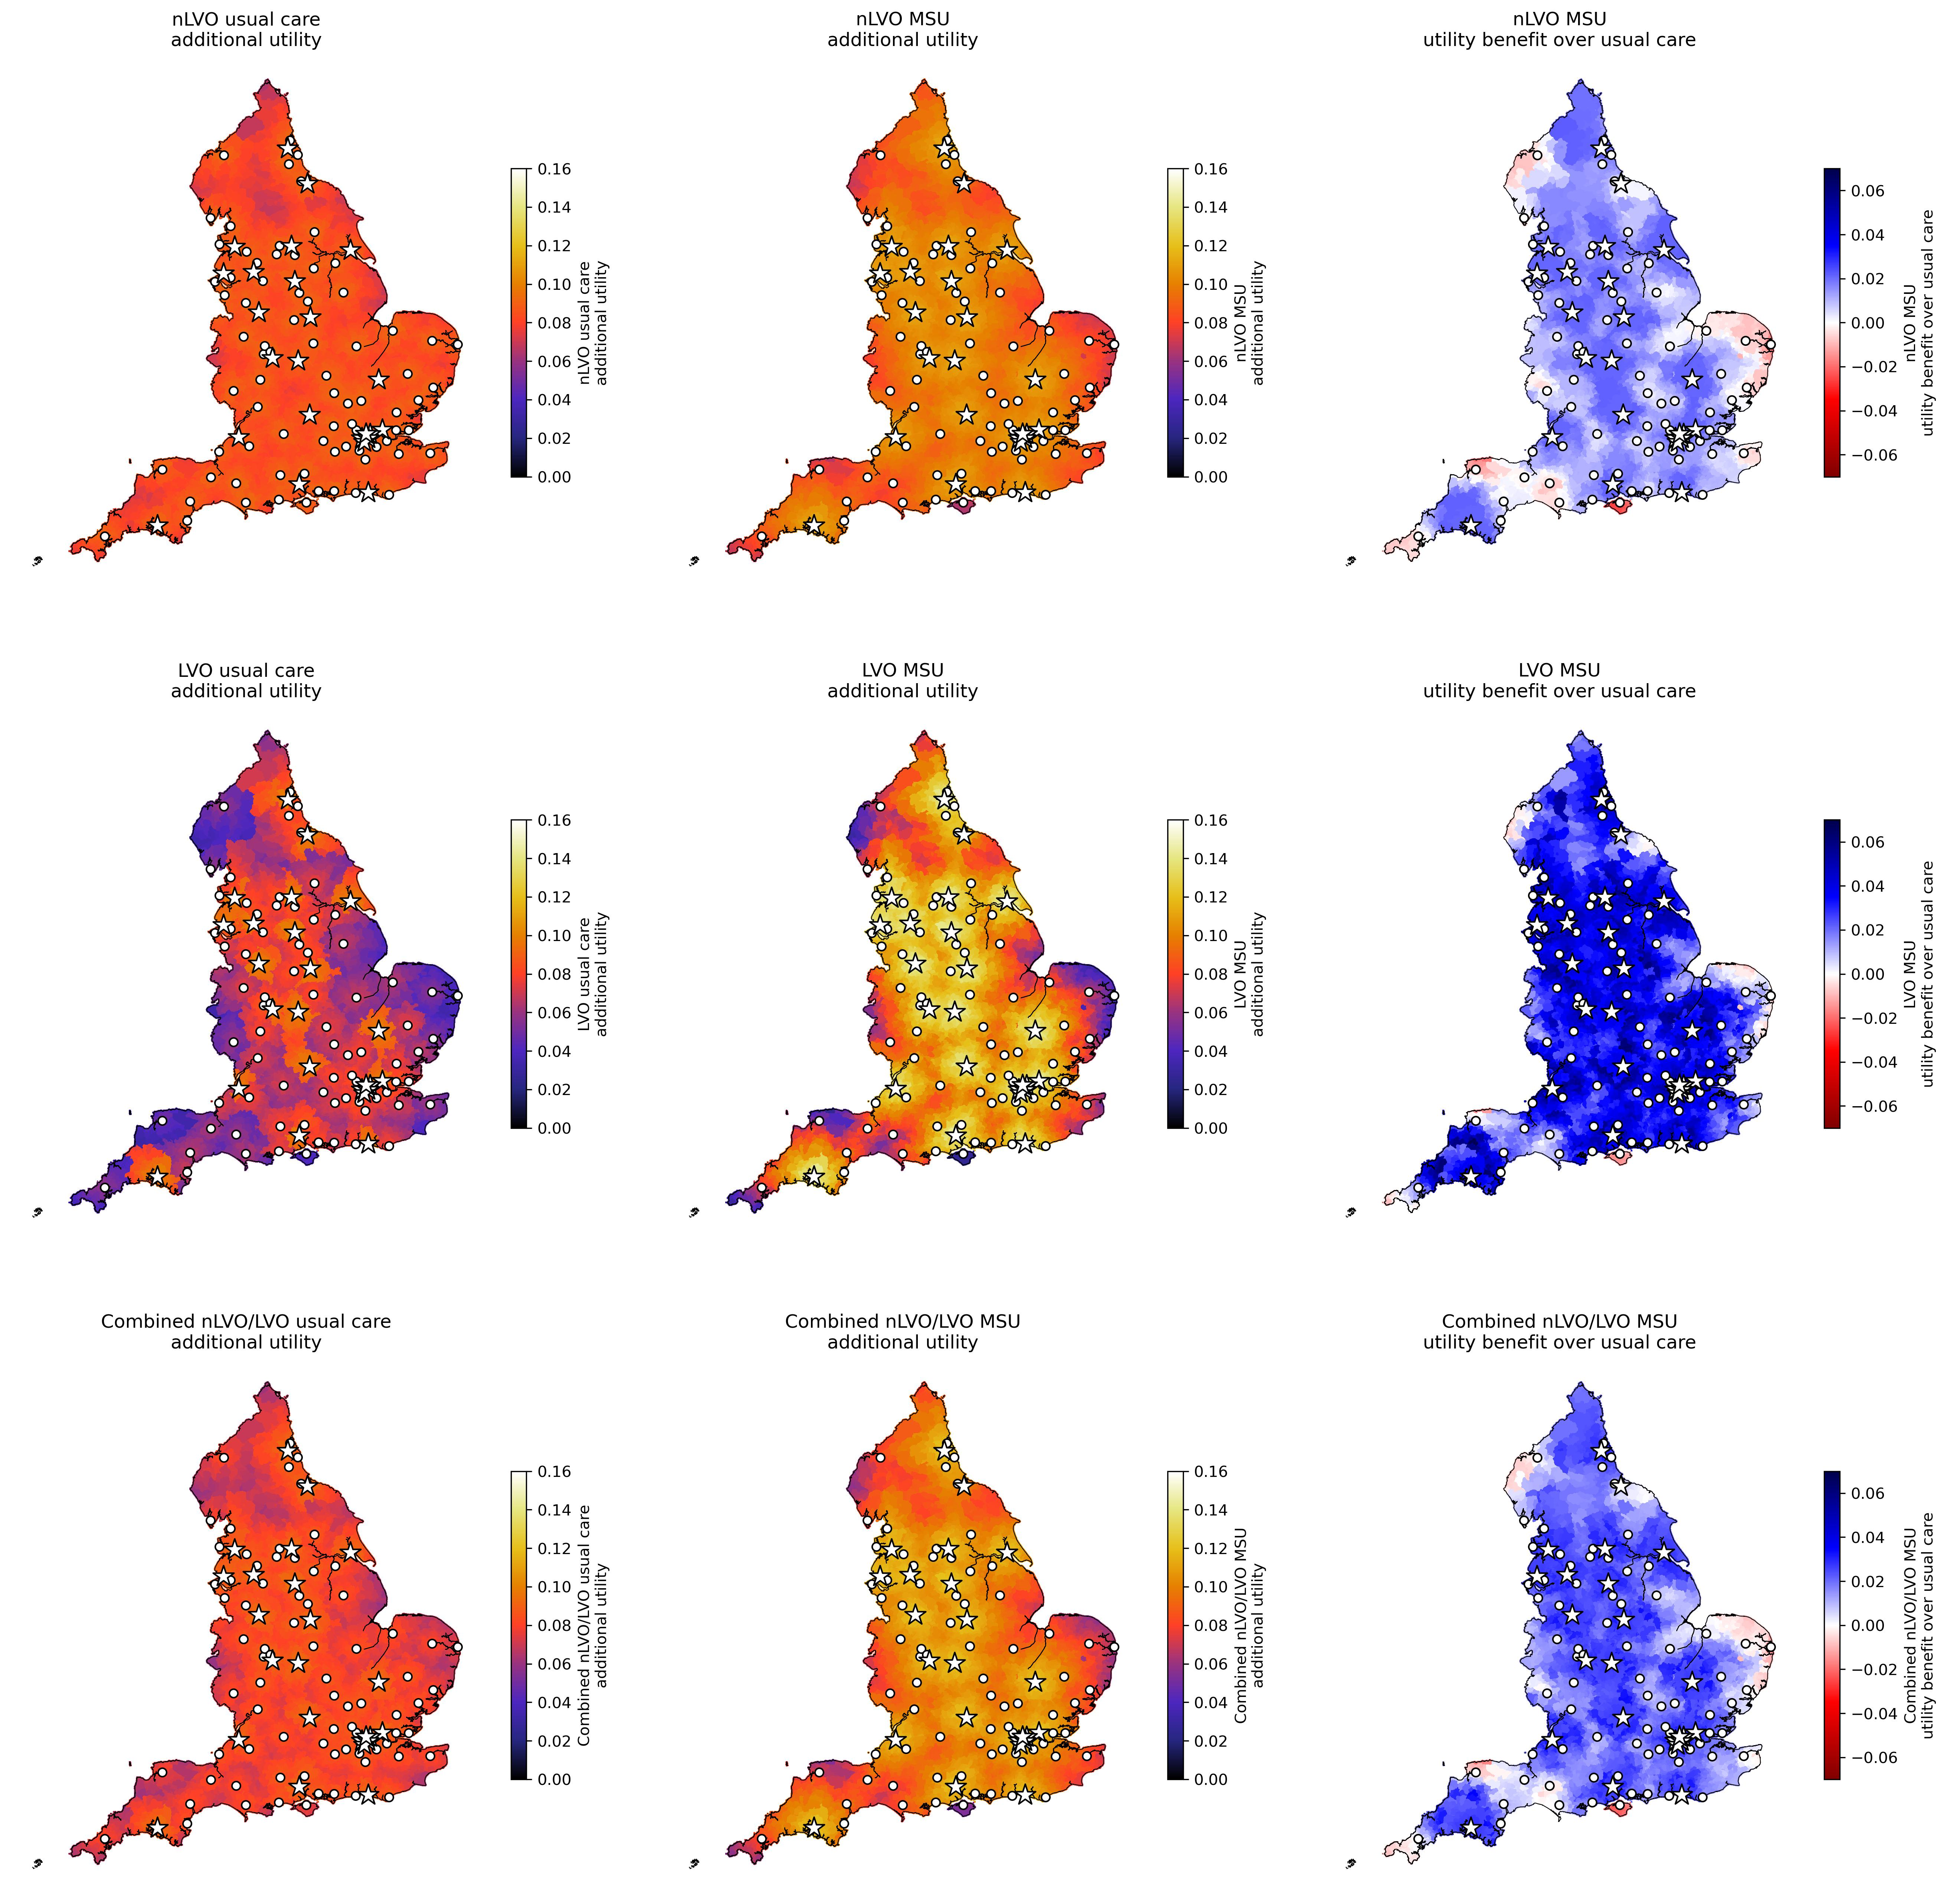
\includegraphics[width=1\linewidth]{images/map_utility.jpg}
    \caption{Map of treatment benefits expressed as the  utility benefit, calculated by LSOA for the treated population. \textit{Top}: Treatment of nLVO; \textit{Middle}: Treatment of LVO, \textit{Bottom}: Combination of treatment (based on 70\% nLVO and 30\% LVO in the treated population, with LVO receiving IVT/MT in combination). \textit{Left}: Benefit of usual care over no treatment; \textit{Middle}: Benefit of MSU care over no treatment; \textit{Right}: Benefit of MSU care over usual care. Circles show locations of PSCs (providing only IVT). Stars show locations of CSCs (providing both IVT and MT, and are also the base locations of MSUs).}
    \label{fig:msu_map_utility}
\end{figure}


Figure \ref{fig:msu_histograms} shows histograms of benefit of MSU care over usual care for the modelled population, with benefit represented as time to treatment, proportion of patients with outcome mRS 0--2 after stroke, and utility. For most LSOAs MSU care improves the time to IVT and MT, but some areas have worsened times. This is reflected in most areas having a benefit of about a 0.03 increase in the proportion of patients with mRS 0--2 after stroke, and similarly a benefit of about a 0.03 increase in utility after stroke. Some areas though have reduced benefit, or even disbenefit of using MSUs. The maximum benefit is about 0.04 improvement in both the proportion of patients with mRS 0--2 after stroke and utility after stroke.

\begin{figure}[h]
    \centering
    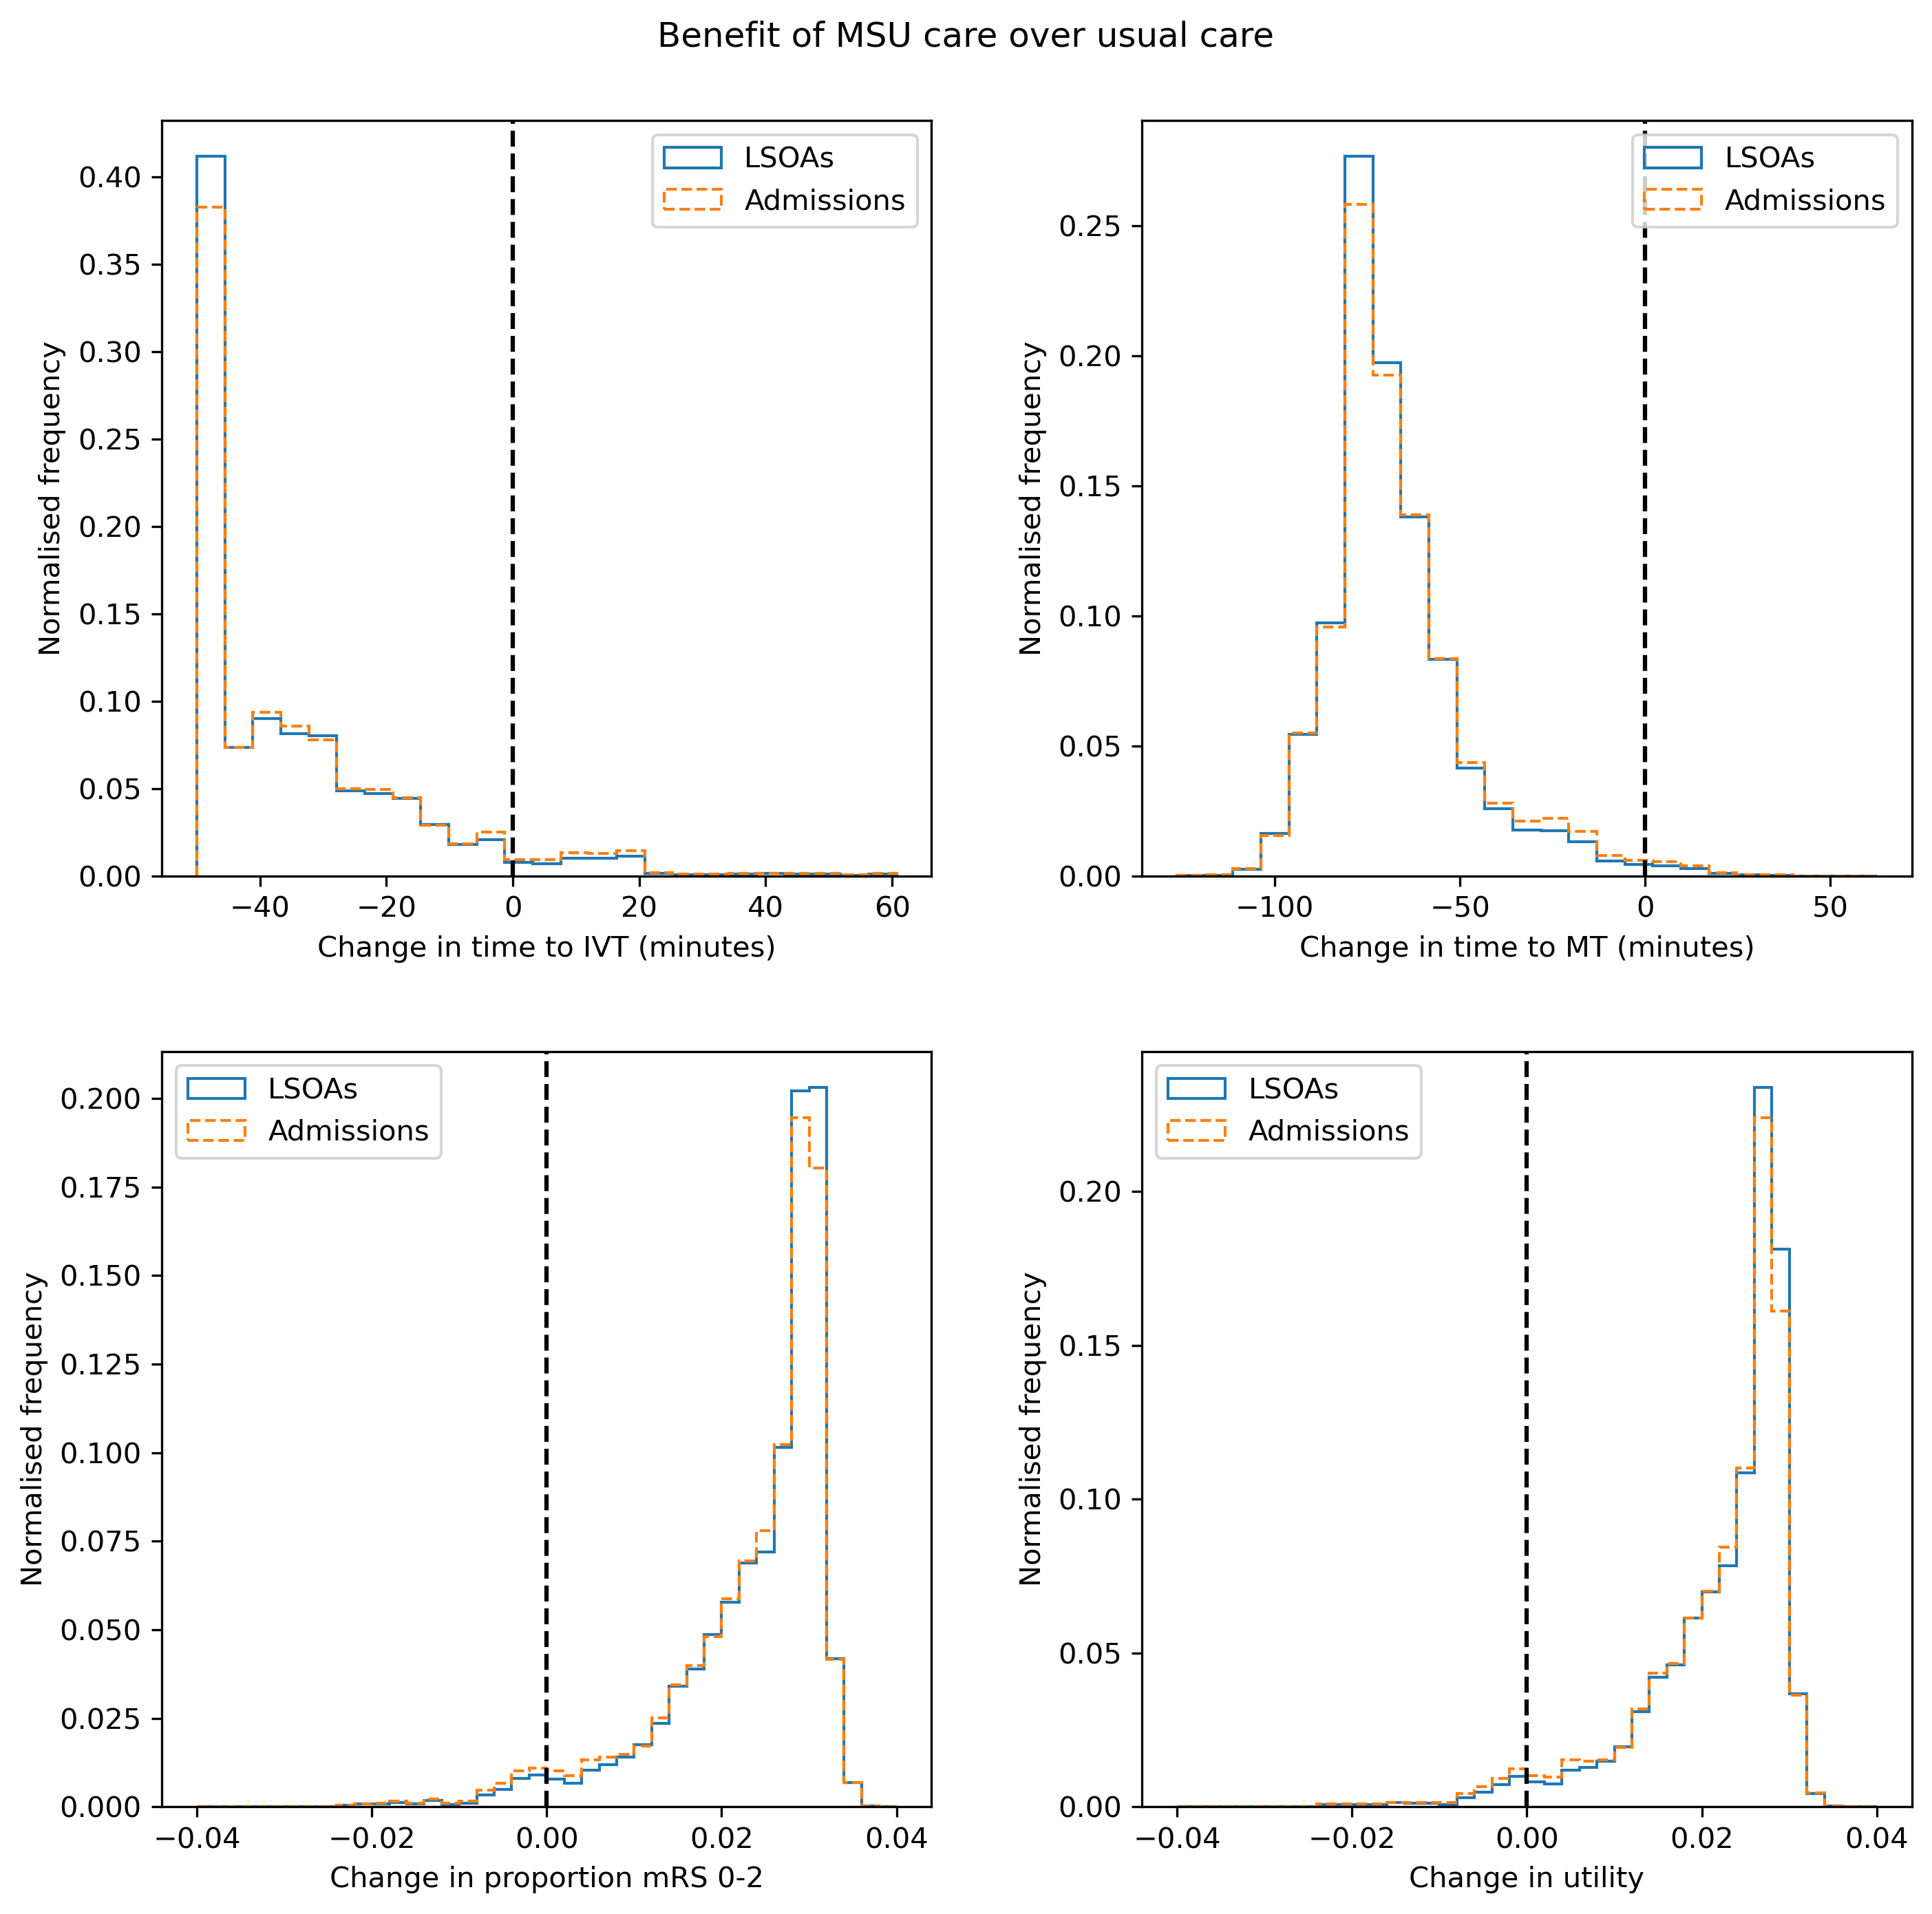
\includegraphics[width=0.75\linewidth]{images/histograms.png}
    \caption{Distribution of benefit of MSU care over usual care across LSOAs (assuming 70\% nLVO, 30\% LVO in the treated population, with LVO receiving IVT/MT in combination). Benefit is described either as even across LSOAs (solid line), or weighted by admissions by LSOA (dotted line). Histograms show change in time to IVT (top left), time to MT (top right), proportion mRS 0--2 post stroke (bottom left), or utility (bottom right).}
    \label{fig:msu_histograms}
\end{figure}

\subsection{Varying number of MSU base locations}

A greedy algorithm was used to select MSU base locations in which MSU base locations are sequentially added one at a time, with each new location selected based on the best possible improvement in utility by adding one more unit. The utility gain is calculated for those patients treated by an MSU rather than with usual care. As the number of MSU base locations increased, the benefit of MSU care over usual care increased (figure \ref{fig:greedy}), but with diminishing returns. The advantage of MSU care over usual care improved utility by 0.020, 0.024, 0.027, and 0.29 with 10, 25, 50 and 100 MSU base locations when MSU base locations are chosen from any stroke unit type. There were 3 CSCs in the first 10 selections, and 8 CSCs in the first 20 selections. With MSU base locations at the 23 current CSCs, the net utility benefit over usual care was 0.022. With the same number of MSU base locations being selected from any stroke centre type, the utility benefit can be increased to 0.023.

\begin{figure}[h]
    \centering
    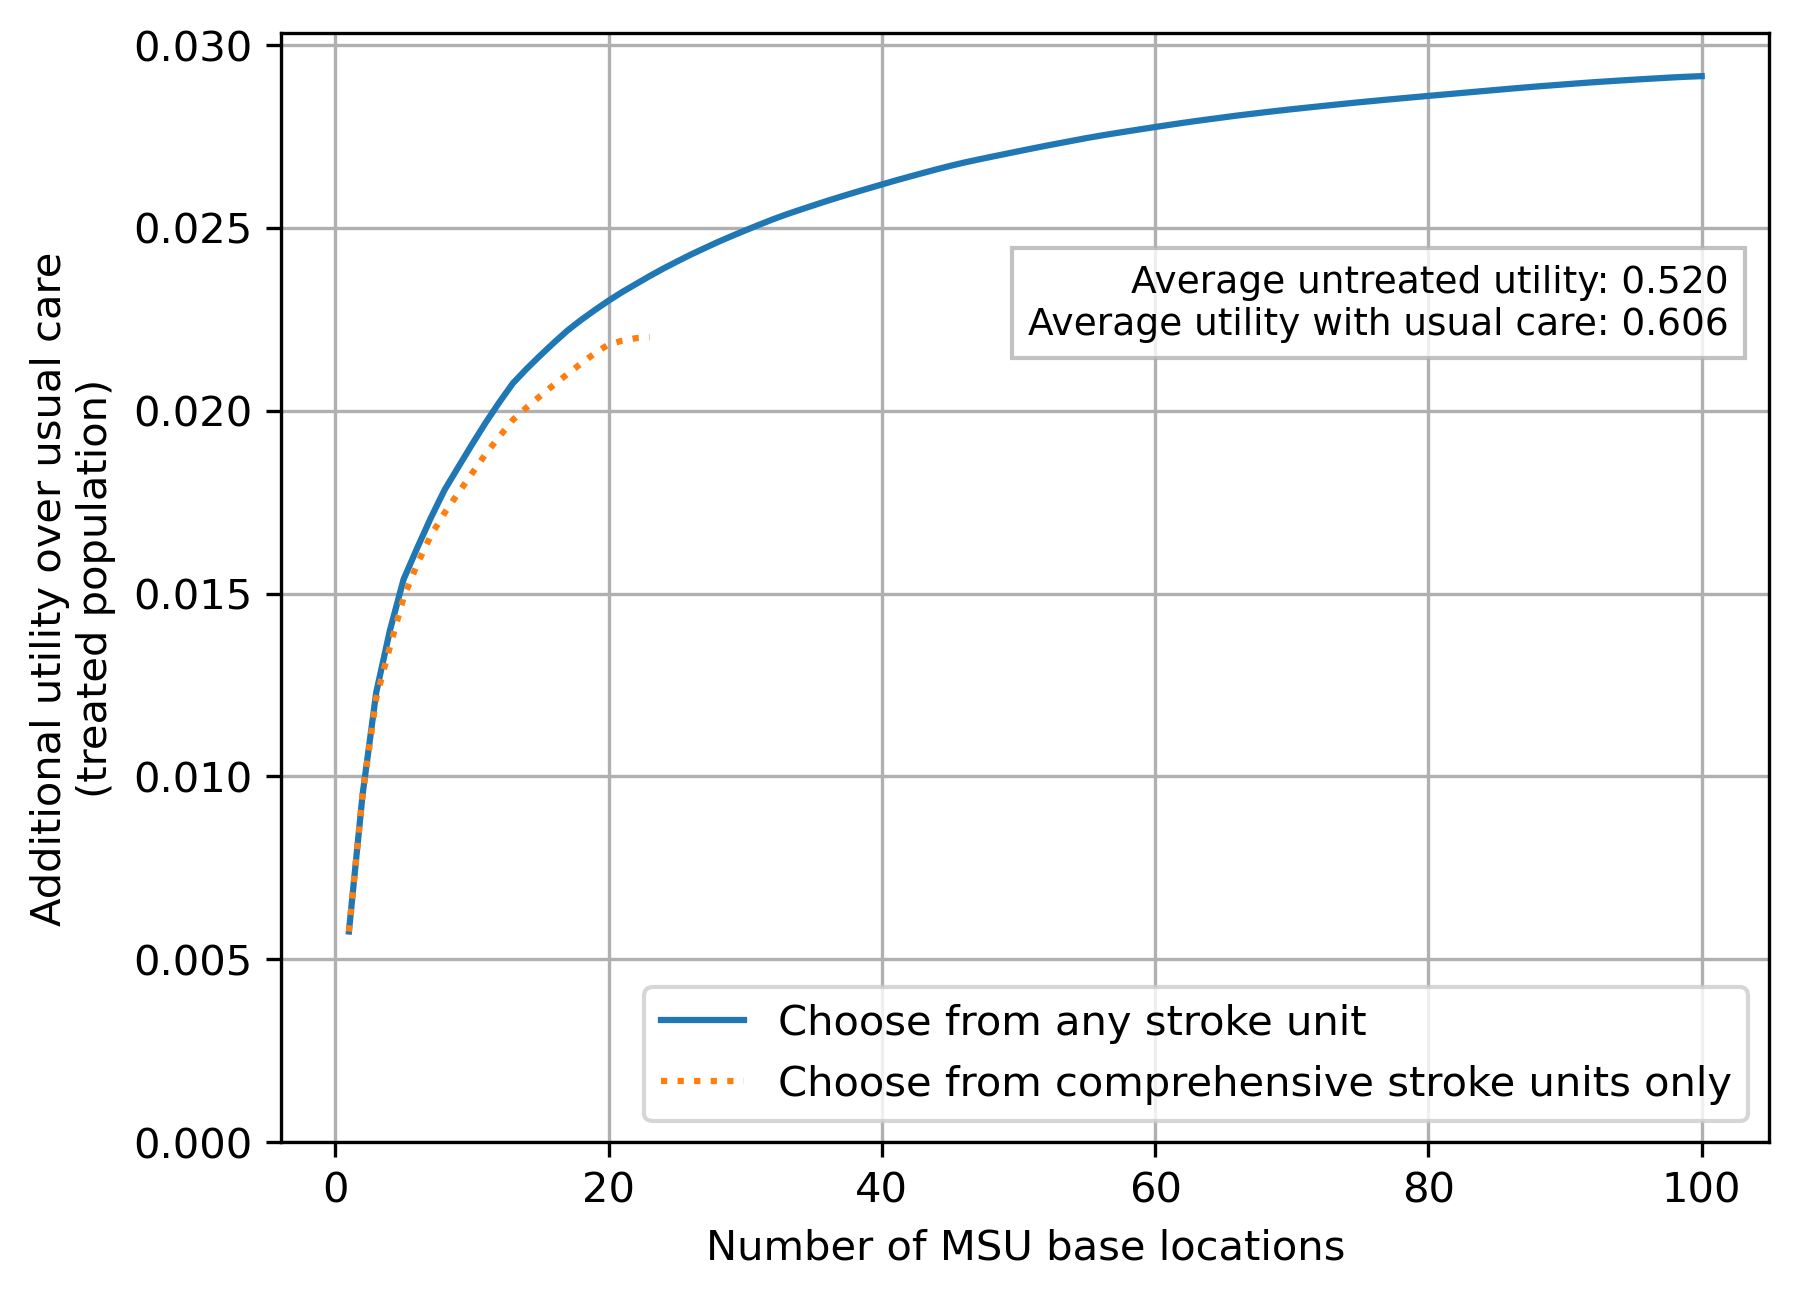
\includegraphics[width=0.5\linewidth]{images/msu_advantages_greedy.png}
    \caption{Increasing number of MSU base locations, with selection by a greedy algorithm based on improvements in utility. The additional utility is for those patients treated by MSU rather than usual care. Units were chosen either from any stroke centre type (solid line) or only from CSCs (dashed line). Utility for the untreated population was 0.520, which was increased to 0.602 with usual care.}
    \label{fig:greedy}
\end{figure}

\subsection{Proportion of patients receiving reperfusion}

In our modelling we have focussed on the benefit for those who receive IVT or MT. Overall, the central probability across realistic scenarios is one extra independent-living outcome for every 50 patients treated. IVT and MT rates vary significantly between countries \cite{kim_global_2024}, but we might take a realistic target of 20\% of patients receiving IVT or MT, in which case there would be one extra independent-living outcome for every 250 confirmed stroke patients (ischaemic and haemorrhagic) where the MSU is dispatched. Not all patients suspected of having stroke at ambulance dispatch will have a confirmed stroke; positive predicted value of suspected stroke at emergency dispatch is about 50\% \cite{kim_global_2024}, in which case there would be one extra independent-living outcome for every 500 of all patients to whom the MSU is dispatched.
